\newpage
\section{Questão 12-34}

\begin{figure}[H]
	\centering
	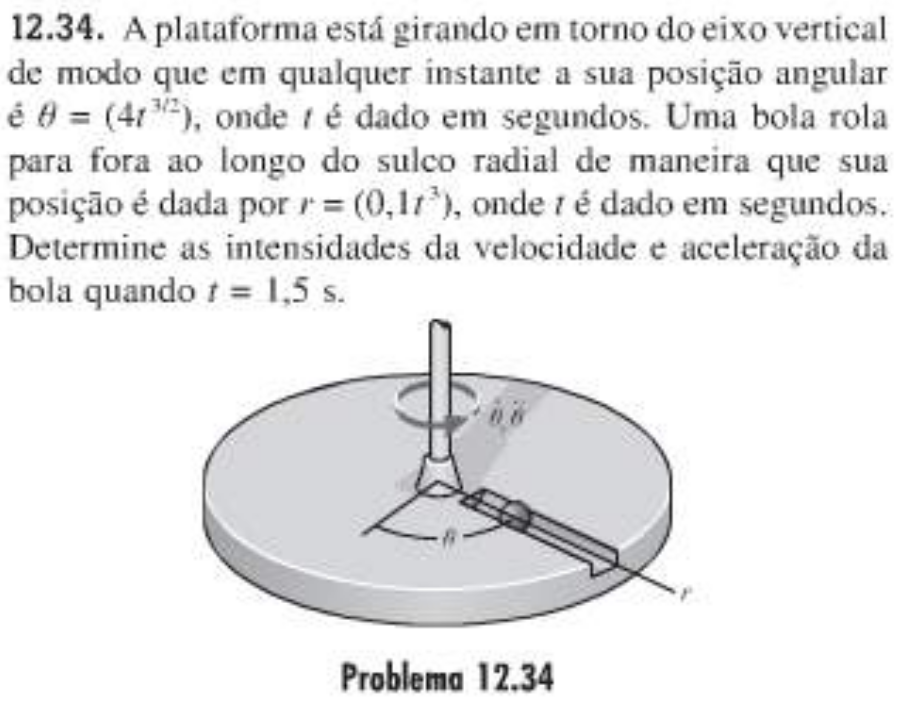
\includegraphics[width=.7\linewidth]{fundamentais/12-34.png}
	\caption{Comando da questão 12-34.}\label{fig:12-34}
\end{figure}


Nesta questão, analisamos o movimento de uma partícula em coordenadas polares, onde a posição radial e a posição angular variam com o tempo. A posição radial é dada por \(r(t) = 0.1 \cdot t^3\), e a posição angular é \( \theta(t) = 4 \cdot t^{3/2}\). Calculamos as velocidades, acelerações e suas intensidades no instante \(t = 1.5 \, \text{s}\).

\subsection*{Velocidade Radial e Angular}
A velocidade radial é a derivada de \(r(t)\) em relação ao tempo:
\[
\frac{dr}{dt} = \frac{d}{dt}\left(0.1 \cdot t^3\right) = 0.3 \cdot t^2.
\]

E a segunda derivada é:
\[
\frac{d^2r}{dt^2} = \frac{d^2\left(0.3t^2\right)}{dt^2} = 0.6t
\]

A velocidade angular é a derivada de \(\theta(t)\) em relação ao tempo:
\[
\frac{d\theta}{dt} = \frac{d}{dt}\left(4 \cdot t^{3/2}\right) = 6 \cdot t^{1/2}.
\]

E sua respectiva segunda derivada é:

\[
\frac{d^2\theta}{dt^2} = \frac{d^2\left(6\cdot t^{1/2}\right)}{dt^2} = 3\cdot t^{-1/2}
\]

\subsection*{Velocidade Tangencial e Intensidade da Velocidade Total}
A velocidade tangencial é dada por:
\[
v_{\text{tangencial}} = r \cdot \frac{d\theta}{dt}.
\]

Substituímos \(r(t) = 0.1 \cdot t^3\) e \(\frac{d\theta}{dt} = 6 \cdot t^{1/2}\):
\[
v_{\text{tangencial}} = \left(0.1 \cdot t^3\right) \cdot \left(6 \cdot t^{1/2}\right) = 0.6 \cdot t^{7/2}.
\]

A intensidade da velocidade total é:
\[
v_{\text{total}} = \sqrt{\left(\frac{dr}{dt}\right)^2 + v_{\text{tangencial}}^2}.
\]

Substituímos \(\frac{dr}{dt} = 0.3 \cdot t^2\) e \(v_{\text{tangencial}} = 0.6 \cdot t^{7/2}\):
\[
v_{\text{total}} = \sqrt{\left(0.3 \cdot t^2\right)^2 + \left(0.6 \cdot t^{7/2}\right)^2}.
\]

\subsection*{Acelerações Radial e Tangencial}
A aceleração radial (centrípeta) é dada por:

\[
a_{\text{radial}} = \frac{d^2r}{dt^2} - r\cdot \left(\frac{d\theta}{dt}\right)^2
\]


Substituímos \(r(t) = 0.1 \cdot t^3\), \(\frac{d^2r}{dt^2} = 0.6t\) e \(\frac{d\theta}{dt} = 6 \cdot t^{1/2}\):
\[
a_{\text{radial}} = \left(0.6t\right) - 0.1t^3 \cdot (6 t^{1/2})^2 = 0.6t - 3.6t^4.
\]


A aceleração tangencial em relação ao tempo vale:
\[
a_{\text{tangencial}} = r \frac{d^2\theta}{dt^2} + 2\frac{dr}{dt}\cdot \frac{d\theta}{dt}
\]

\[
a_{\text{tangencial}} = 0.1t^3 \cdot 3t^{-1/2} + 2\cdot 0.3t^2\cdot 6t^{1/2} = 0.3t^{5/2} + 3.6 t^{5/2} = 3.9 t^{5/2}
\]

A intensidade da aceleração total é:
\[
a_{\text{total}} = \sqrt{a_{\text{radial}}^2 + a_{\text{tangencial}}^2}.
\]

Substituímos \(a_{\text{radial}} = 0.6t - 3.6 \cdot t^4\) e \(a_{\text{tangencial}} = 3.9 \cdot t^{5/2}\):
\[
a_{\text{total}} = \sqrt{\left(0.6t - 3.6 \cdot t^4\right)^2 + \left(3.9 \cdot t^{5/2}\right)^2}.
\]

\subsection*{Cálculos no Instante \(t = 1.5 \, \text{s}\)}
Substituímos \(t = 1.5 \, \text{s}\) nas expressões:
\begin{itemize}
    \item Velocidade total:
    \[
    v_{\text{total}} = \sqrt{\left(0.3 \cdot 1.5^2\right)^2 + \left(0.6 \cdot 1.5^{7/2}\right)^2} \approx 2.57032 \, \text{m/s}.
    \]
    \item Aceleração total:
    \[
    a_{\text{total}} = \sqrt{\left(3.6 \cdot 1.5^4\right)^2 + \left(2.1 \cdot 1.5^{5/2}\right)^2} \approx 20.3877 \, \text{m/s}^2.
    \]
\end{itemize}